\documentclass[11pt]{article}
\usepackage[margin=1in]{geometry}
\usepackage{amsmath,amssymb}
\usepackage{graphicx}
\usepackage{booktabs}
\usepackage{microtype}
\usepackage[numbers,sort&compress]{natbib}
\usepackage{xcolor}
\usepackage[colorlinks=true,allcolors=blue]{hyperref}

\title{\textbf{When Does Learning Beat Reflexes?\\
A Pre-Registered Study of Reinforcement Learning vs.\ Classical Control at the Friction Limit}}

\author{Edward \\ \textit{AutoDrift Project} \\ \texttt{edwardoptimization@gmail.com}}
\date{Preprint --- \today}

\begin{document}
\maketitle

\begin{abstract}
Reflex and classical controllers are excellent in benign regimes but cannot operate in
saturated, unstable-equilibrium regimes such as sustained drift, where the tyres are past peak
grip and the vehicle balances on an unstable saddle of the sideslip--yaw dynamics. We ask a
bounded question: \emph{where}, and \emph{why}, does a learned policy beat classical control?
We answer it under pre-registered, five-arm adjudication in a high-fidelity multibody simulator.
A single deployable policy (a 72-dimensional observation mapped to a 3-dimensional action by an
asymmetric actor--critic, behaviour-cloning warm-start followed by PPO, with gated dual output
heads) \emph{reliably surpasses both a reflex floor (success $0.00$) and a hand-tuned feedback
oracle ($0.35$) on drift} ($0.856$, seed-clustered $95\%$ CI $[0.728,\,0.953]$, $16$ seeds),
while it \emph{regresses on the easy avoidance regime} ($0.700$ vs.\ a trivial classical floor of
$1.00$, CI of the difference $[-0.500,\,-0.125]$). We characterise this regime tradeoff rather
than hide it. Two findings support the result. First, a long history of ``RL cannot drift''
negatives traces to two identifiable training bugs (an under-trained warm-start and a
selection-timing error), not to a fundamental limit. Second, the avoidance regression is
cross-regime gradient interference on shared policy weights; we rule out smoothing, capacity, and
gradient surgery, and partly resolve it with gated dual heads that give each regime its own output
weights. The contribution is a rigorous, honestly bounded answer: at the friction limit learning
wins decisively; in the benign regime it should not replace classical control.
\end{abstract}

\section{Introduction}
A self-driving controller spends almost all of its time in a benign regime---moderate speeds,
tyres well within their linear range---where decades of classical and reflex control deliver near
perfect behaviour. The hard cases live elsewhere: at the limit of friction, where a manoeuvre
demands operating tyres past peak grip and stabilising the vehicle on an unstable equilibrium.
Sustained drift is the canonical example. The sideslip--yaw dynamics of a vehicle with nonlinear
tyres have unstable saddle equilibria at high sideslip; holding one requires coordinated steering
and throttle and tolerates no sustained error, because small action mistakes compound and spin the
car out within a fraction of a second~\citep{velenis2010analysis,goh2020toward}. Reflex controllers
tuned for the benign regime do not operate here at all.

This invites a sharp, falsifiable question that is more useful than the usual ``can RL drive?'':
\emph{where, and why, does a learned policy beat classical control, and where does it not?} We
study it for a single policy that must handle two regimes with one set of weights---sustained drift
(hard, at the limit) and obstacle avoidance (easy, solved trivially by classical control)---and we
hold ourselves to a pre-registered, five-arm comparison frozen before any training run.

Our answer is two-sided and, we believe, the honest one. On drift, the learned policy is decisively
better than both the best learning-free classical arm and a hand-tuned feedback oracle, with
seed-clustered confidence intervals that exclude zero by a wide margin. On avoidance, the same
policy is significantly \emph{worse} than a trivial classical controller. We do not average these
away. Instead we trace each to its cause: the drift capability was unlocked by fixing two concrete
training bugs, and the avoidance regression is gradient interference between the two regimes on the
shared policy weights, which we localise and partly resolve.

\paragraph{Contributions.}
\begin{enumerate}
  \item A pre-registered, five-arm empirical result in a high-fidelity multibody simulator showing
  that a single learned policy reliably beats both a reflex floor and a hand-tuned oracle in the
  saturated drift regime ($0.856$ vs.\ $0.00$ and $0.35$; $16$ seeds; CI excludes zero), while
  honestly regressing on the benign avoidance regime.
  \item A root-cause analysis showing that ``RL cannot drift'' negatives were two identifiable
  training bugs, not a representational or task limit.
  \item A lever-elimination study of the regime tradeoff that localises the conflict to shared
  output weights (via gradient surgery) and partly resolves it with gated dual output heads.
\end{enumerate}

\section{Related Work}
\paragraph{Reinforcement learning for drifting and at-the-limit racing.}
Deep RL has produced impressive drift and racing controllers. \citet{cai2020high} train a
high-speed drift policy in simulation with an error-and-derivative observation and a sideslip-,
heading-, and path-error reward, with heavy in-environment action smoothing.
\citet{wurman2022outracing} reach champion-level Gran Turismo lap times with a distributional critic
and very large-scale off-policy data. Recent work transfers drift policies to hardware: a learned
individual-wheel-drive policy with massive GPU parallelism and domain randomisation~\citep{zhou2025learning},
and a reference-free formula-drift controller that replaces domain randomisation with an
uncertainty-aware learned vehicle model~\citep{djeumou2024reference}. These works demonstrate
\emph{that} RL can drift and race; we ask the complementary, pre-registered question of \emph{where and
why} a learned policy beats classical control, and we report the benign-regime cost rather than only
the at-the-limit win.

\paragraph{Drift-equilibrium theory and classical control.}
Model-based analyses establish that drift equilibria are unstable saddle points reached in a
countersteer configuration, and---important for our design---that they have low sensitivity to
friction and speed~\citep{velenis2010analysis,goh2020toward}. This is why a policy that never
observes the friction coefficient can still stabilise drift: the equilibrium it must hold is
nearly friction-invariant. These works are model-based and serve as the theoretical backdrop, not
as learning baselines.

\paragraph{Asymmetric and privileged learning, adaptation, and multi-task interference.}
Training a deployable proprioception-only policy with a privileged critic or teacher is standard in
legged locomotion~\citep{lee2020learning,chen2020learning,kumar2021rma}; our actor reads only the
deployable observation while the critic sees privileged channels at train time. Domain
randomisation and its automatic variants~\citep{tobin2017domain,peng2018sim,openai2019solving}
train one policy over a distribution rather than enumerating a grid. When one policy serves multiple
tasks, gradients can conflict; gradient surgery projects away the conflicting component~\citep{yu2020gradient}.
We use the latter not as a fix but as a diagnostic that localises our regime conflict to the shared
output weights.

\section{Problem Setup}
\paragraph{Regimes and the policy interface.}
The agent controls a vehicle in two regimes. In \emph{drift}, it must enter and sustain a
controlled high-sideslip slide on a low-friction surface for at least a fixed number of steps; the
episode starts already near the drift equilibrium (sideslip $\beta_0 = 0.22$\,rad, target
$\beta^\star = 0.28$\,rad). In \emph{avoidance}, it must avoid an obstacle revealed at a range
drawn from a frozen grid across friction levels. A single policy maps a $72$-dimensional
deployable observation (vehicle kinematics, boundary and obstacle features---\emph{no} friction or
regime label) to a $3$-dimensional action (steering, throttle, brake). The deployable policy is the
actor only.

\paragraph{Simulator.}
We use Project Chrono~\citep{projectchrono}, a high-fidelity multibody engine, with a TMeasy-tyre
sedan stepping its internal dynamics at \mbox{$1$\,kHz} behind a $50$\,Hz control interface. The
nonlinear tyre and load-transfer model is what makes the saturated drift regime meaningful; it also
makes the simulator CPU-bound, a constraint we return to in the discussion.

\paragraph{Five-arm adjudication and pre-registration.}
Following a pricing discipline, we compare the learned \emph{student} against four learning-free or
oracle arms: a fixed reflex controller, an entry-speed-commitment floor, an online friction-seeker
floor, and a per-regime \emph{oracle} (a hand-tuned feedback law, the best non-learning controller
we could build for each regime). The floor is the maximum over the non-trivial classical arms---not
a strawman. The entire protocol---success criteria, the five arms, a reward-alignment gate, an
oracle-ceiling stop rule, the validation seeds, and seed-clustered confidence intervals---was frozen
before the confirmatory run. We report per-regime success on $30$ frozen validation episodes per
regime, aggregated over $16$ training seeds, with $95\%$ confidence intervals computed by clustering
on the training seed (a paired-$t$ interval and a cluster bootstrap as robustness).

\section{Method}
\paragraph{Asymmetric actor--critic with warm-start then PPO.}
The actor is a Gaussian policy over the $72$-dimensional observation with a learnable per-action
log-standard-deviation; deployment uses the squashed mean. The critic additionally reads six
privileged channels (true friction, mass and grip surrogates, reveal distance, and a regime
one-hot) used only during training. We warm-start the actor by behaviour cloning the per-regime
teacher laws, then refine with PPO~\citep{schulman2017proximal} using a bootstrapped privileged
GAE critic and per-regime advantage normalisation. Checkpoints are selected on task success on a
disjoint evaluation set, never on the teacher-imitation loss.

\paragraph{Two bugs behind ``RL cannot drift''.}
A long line of negatives in this project had concluded that the drift regime was not learnable.
We trace those to two concrete training bugs. First, the behaviour-cloning warm-start ran for a
single epoch; the under-trained imitation could not reach the action precision a drift saddle
demands, so PPO began from a near-random policy and stalled. A converged warm-start removes this.
Second, the task-score checkpoint selection only evaluated the policy \emph{after} each PPO update;
with many parallel rollout workers the first update could move the warm-start policy substantially,
so the converged warm-start checkpoint was never an eligible candidate. Capturing the warm-start as
a candidate \emph{before} the first PPO update fixes this. Neither bug is about representation or
task feasibility: a converged warm-start alone already drifts.

\paragraph{Regime interference and gated dual heads.}
With drift learnable, the open problem becomes the avoidance regression. We show it is gradient
interference: the drift and avoidance policy gradients conflict on the shared actor output weights,
so improving drift corrupts avoidance-state outputs. We eliminate alternatives in turn. An
input-Jacobian penalty (smoothing the policy) is null-to-negative. Adding actor capacity is ruled
out a priori---a capacity sweep shows behaviour-cloning fit saturates at a small hidden width and
deeper networks hurt. Gradient surgery~\citep{yu2020gradient} rebalances the tradeoff frontier
(more avoidance, less drift) but cannot expand it, which localises the conflict to the shared output
weights. We then give each regime its own output head: a shared trunk feeds two action-mean heads
blended by a learned soft gate (a sigmoid that infers the regime from the observation, since the
regime label is privileged and unavailable to the deployable policy). Separate output weights cannot
corrupt one another, and the policy remains a single deployable observation-only actor.

\section{Experiments}
\paragraph{Headline result.}
Table~\ref{tab:main} reports the five-arm adjudication for the $16$-seed gated policy. On drift the
student reaches $0.856$ success with a seed-clustered $95\%$ CI of $[0.728,\,0.953]$; the reflex
floor is $0.00$ and the hand-tuned oracle is $0.35$, so the learned policy beats the best
non-learning controller by more than $0.5$ in absolute success, and the difference from the floor
excludes zero with margin. On avoidance the student reaches $0.700$ against a trivial classical
floor of $1.00$; the CI of the difference is $[-0.500,\,-0.125]$, a significant regression that we
report as such. Pooled success is $0.762$. All pre-registered protocol gates pass.

\begin{table}[t]
\centering
\caption{Five-arm adjudication, $16$ training seeds, $30$ frozen validation episodes per regime.
Success rate; CI is the seed-clustered $95\%$ interval of (student $-$ floor).}
\label{tab:main}
\begin{tabular}{lccc}
\toprule
 & reflex floor & per-regime oracle & \textbf{learned student} \\
\midrule
drift     & $0.000$ & $0.350$ & $\mathbf{0.856}$ \quad CI $[0.728,\,0.953]$ \\
avoidance & $1.000$ & $1.000$ & $0.700$ \quad CI $[-0.500,\,-0.125]$ \\
pooled    & $0.600$ & $0.740$ & $0.762$ \\
\bottomrule
\end{tabular}
\end{table}

\paragraph{The negatives were bugs (ablation).}
A converged behaviour-cloning warm-start, alone, drifts where the one-epoch warm-start cannot; and
capturing that warm-start as a selection candidate before the first PPO update is what lets the
final policy keep it when PPO degrades a given seed. Both are single-line changes with large,
reproducible effects, and neither involves more capacity, more data, or a different observation.

\paragraph{Lever elimination for the regime tradeoff.}
Figure~\ref{fig:levers} contrasts the candidate fixes against the single-head baseline (drift
$0.769$, avoidance $0.775$). An input-Jacobian penalty is null-to-negative and widens the avoidance
CI. Gradient surgery moves \emph{along} the frontier (avoidance up to $0.863$, drift down to
$0.556$) without expanding it. Gated dual heads are the only lever that expands the frontier: drift
rises to $0.925$ (at eight seeds) with avoidance held, and to $0.856$ under the harder $16$-seed
sample. The eight-seed avoidance CI touched zero; sixteen seeds reveal the regression is real, which
is the statistical-hardening result behaving as intended.

\begin{figure}[t]
\centering
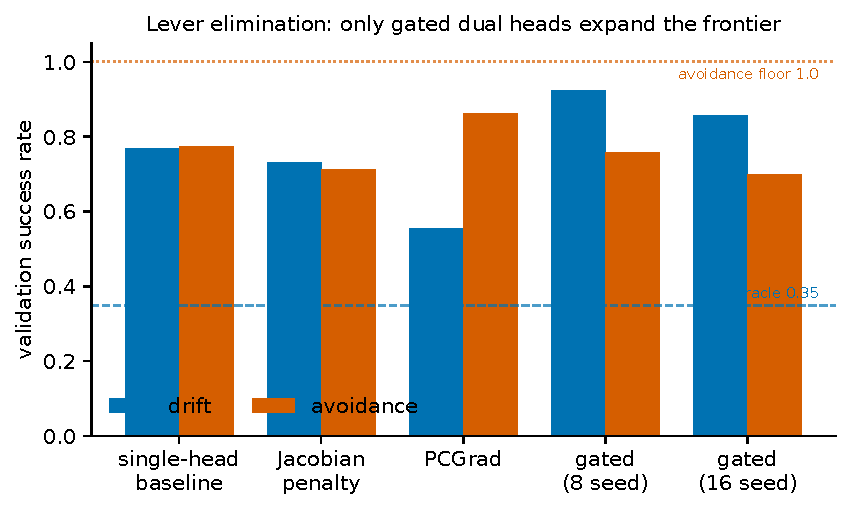
\includegraphics[width=0.86\linewidth]{figs/fig2_levers}
\caption{Lever elimination. Each pair of bars is a full confirmatory run that differs only in
the named intervention (8 seeds unless noted; ``gated (16 seed)'' is the canonical run). The
input-Jacobian penalty is null-to-negative; gradient surgery (PCGrad) moves \emph{along} the
tradeoff frontier (avoidance up, drift down); only gated dual heads \emph{expand} it (drift up,
avoidance held). Dashed line: the drift oracle ($0.35$); dotted line: the avoidance floor ($1.0$).}
\label{fig:levers}
\end{figure}

\paragraph{Per-seed frontier.}
We ask, per seed, whether any single checkpoint achieves both regimes well (drift and avoidance
each $\geq 0.75$; the ``both-good'' region in Figure~\ref{fig:frontier}). The single-head policy
reaches this for $3/8$ seeds; the gated policy reaches it for $8/16$. The remaining seeds either
cannot drift or collapse avoidance when drift is high---a genuine tradeoff that gated heads reduce
but do not eliminate, and the reason the aggregate avoidance still regresses.

\begin{figure}[t]
\centering
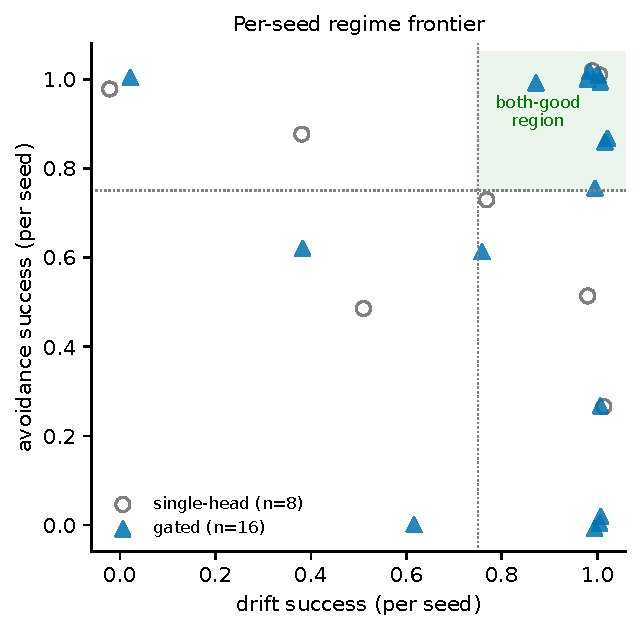
\includegraphics[width=0.62\linewidth]{figs/fig3_frontier}
\caption{Per-seed regime frontier: the selected checkpoint's drift vs.\ avoidance success, one
marker per training seed (points jittered to separate coincident discrete values). Gated heads
move more seeds into the both-good region (top-right, drift and avoidance $\geq 0.75$): $8/16$ vs.\
$3/8$ for the single-head policy. Seeds outside it either cannot drift (left) or trade avoidance
for drift (bottom-right).}
\label{fig:frontier}
\end{figure}

\section{Discussion and Limitations}
The result is bounded by design, and the boundaries are the point. \emph{Where} learning wins is
the saturated drift regime, in which it beats both reflex control and a hand-tuned oracle reliably
across seeds. \emph{Where} it should not be used is the benign avoidance regime, in which a trivial
classical controller is strictly better and the learned policy regresses. A deployed system should
therefore prefer classical control in the benign regime and hand off to the learned policy only at
the limit---a conclusion the pre-registered comparison supports directly.

Several limitations are explicit. The study is simulation-only; we make no real-vehicle transfer
claim. The avoidance regression is real and significant at sixteen seeds; gated heads make the
\emph{drift} win reliable, not the avoidance regime. The per-seed analysis suggests the residual is
partly fundamental and partly a training-variance effect: only half the seeds reach a
both-regimes-good checkpoint, and the CPU-bound simulator caps the rollout batch far below the
thousands of parallel environments used in GPU-native drift work~\citep{zhou2025learning,djeumou2024reference},
which is the suspected reason more seeds do not reach the both-good frontier. Reducing that variance
(more parallel data, or a learned GPU-batched surrogate of the multibody simulator) is the clearest
route to making both regimes reliable, and is the natural next step.

\section{Conclusion}
At the friction limit, learning wins: a single deployable policy reliably beats both reflex control
and a hand-tuned oracle on sustained drift, under a pre-registered, five-arm comparison. In the
benign regime it does not, and we report that honestly. The drift capability was unlocked by fixing
two concrete training bugs, and the regime tradeoff was localised to shared output weights and
partly resolved with gated dual heads. The useful claim is not ``RL drives,'' but a bounded map of
\emph{where} and \emph{why} learning beats reflexes---and where it does not.

\paragraph{Reproducibility and AI-use disclosure.}
The protocol was pre-registered and frozen before the confirmatory run; results, the frozen
preregistration, and the full method log are in the project repository. The lever-elimination
interventions are toggleable and off by default, so the canonical pipeline is reproducible from the
default configuration. This manuscript was drafted with AI assistance (an automated paper-writing
pipeline); all numbers are taken from the committed experimental artefacts and all citations were
verified against primary sources by the authors.

\bibliographystyle{unsrtnat}
\bibliography{references}

\end{document}
